\documentclass{article}
\usepackage{amsmath, amssymb}
\usepackage{amsthm}
\usepackage{graphicx}
\newtheorem{theorem}{Theorem}[section]
\newtheorem{lemma}{Lemma}[section]
\newtheorem{conjecture}{Conjecture}[section]
\newtheorem{definition}{Definition}[section]
\newtheorem{remark}{Remark}[section]

\graphicspath{ {./rl-3-ratio/} }

\begin{document}

\title{Observations on Every Third Digit of the Thue-Morse Sequence}
\author{
	Adam Hutchings
	\and
	Henry Hutchings
	\and
	Jake Roggenbuck
}
\maketitle

\begin{abstract}
We investigate some interesting properties of the sequence made up of every third term of the Thue-Morse sequence. Moreover, we create proofs for said properties.
\end{abstract}

\tableofcontents

\section{Introduction}
The Thue-Morse sequence, or $T,$ can be defined in many ways, and we will use the following definition for the $n$th digit of the sequence, denoted by $T(n):$ 
\begin{definition}[Thue-Morse Sequence]
The Thue-Morse sequence is the sequence whose $n$th term $T(n)$ depends on the number of ones in the binary representation of $n.$ If this number is odd, $T(n)$ is $1;$ otherwise, it is $0.$
\end{definition}
The sequence $T_3,$ which is defined as the sequence whose $n$th term is $T(3n),$ has some interesting properties that we will investigate -- among the most interesting of which are the lengths of runs in the sequence and the persistent imbalance of zeroes and ones. We will prove two main results:

\begin{theorem}[Motif Theorem]
\label{mlength}
Motifs in $T_3$ are only of lengths 1, 3, 6, 7, or 8.
\end{theorem}

\begin{theorem}[Imbalance Theorem]
\label{ratio}
The number of zeroes in the first $n$ digits of $T_3$ always exceeds the number of ones for any $n > 0.$
\end{theorem}

We also develop two main techniques to prove these theorems and others -- the segment-matching method and its reverse -- which may be extended in the future to investigate $T_n,$ which is defined so that $T_n(x) = T(nx).$

\section{Run-Length Of $T_3$}

\subsection{Motifs and the $\Lambda$ Function}
We define $segments,$ $runs,$ and $motifs$ in $T_3$ as follows:

\begin{definition}
\label{segment}
A \emph{segment} of length $n$ is $n$ consecutive terms in a sequence.
\end{definition}

\begin{definition}
\label{run}
A \emph{run} of length $n$ is a segment of length $n,$ all of whose terms are identical.
\end{definition}

\begin{definition}
\label{motif}
A \emph{motif} of length $n$ is a run of length $n$ which is not contained inside a run of length $m > n.$
\end{definition}

Similar to the computer science notion of \emph{run-length encoding}, we define a function $\Lambda$ which takes as input a sequence of integers $x$ and outputs another sequence of integers $\Lambda(x)$ whose $n$th term is denoted $\Lambda(x)(n).$ It is defined as follows:

- $\Lambda(x)(0)$ is the length of the motif in $x$ starting at $x(0).$

- $\Lambda(x)(n)$ is the length of the motif starting at the term in $x$ indexed by $\sum_{k=0}^{n-1} \Lambda(x)(k).$

In other words, $\Lambda$ takes as input a sequence of numbers and transforms it into a sequence denoting the lengths of motifs in the input.

\subsection{$\Lambda(T_3)$}

The authors created a computer program to investigate the sequence $\Lambda(T_3)$ and noted that it consists, for all values checked, of only 1, 3, 6, 7, and 8. In other words, length of motifs in $T_3$ consist of only these values. The rest of Section 2 will be devoted to proving this.

\subsection{No-2 Theorem}

\begin{theorem}[No-2 Theorem]
\label{no2}
There are no motifs of length $2$ in $T_3.$ Equivalently, $\Lambda(T_3)$ contains no $2$s.
\end{theorem}

\begin{proof}
We begin by observing that a motif of zeroes of length 2 is the sequence $00$ surrounded by $1$s, and a motif of ones of length 2 is the opposite, except at the beginning of the sequence. However, the sequence $T_3$ begins with a motif of length 7, so this caveat is not necessary. These translate to $1001$ and $0110$ in $T_3,$ which must exist if the No-2 Theorem is false. Because we obtain the elements of $T_3$ from choosing every third element of the Thue-Morse sequence, the existence of $1001$ or $0110$ in $T_3$ implies the existence of $1XX0XX0XX1$ or $0XX1XX1XX0$ in the Thue-Morse sequence where $X$ is either digit.

\begin{lemma}
\label{triplet}
The sequences $000$ and $111$ do not exist in the Thue-Morse sequence.
\end{lemma}

\begin{proof} The non-existence of runs of length 3 in the sequence is a well-known fact, but may be established as follows: jumping from $2n$ to $2n+1$ changes a $0$ to a $1$ and nothing else, which means that $T_{2n}$ and $T_{2n+1}$ are opposite. Therefore, the entire Thue-Morse sequence consists of concatenations of $01$ and $10,$ which allow for no $000$ or $111.$
\end{proof}

Lemma \ref{triplet} allowed for us to create a computer program to comb through all ten-digit sequences of zeroes and ones, with the constraints that they follow the pattern $0XX1XX1XX0$ and do not contain $000$ or $111.$  The only ten-digit sequences that satisfy these constraints are $0011001010,$ $0011001100,$ $0011011010,$$0101001010,$ $0101001100,$ $0101011010,$ $0101101010,$ and $0101101100.$ We do not check for any occurrences of $1001$ in $T_3,$ (which would follow the pattern $1XX0XX0XX1$ in $T$) but this is not necessary, as shown by:

\begin{lemma}
\label{xiffxbar}
A sequence $X$ exists in the Thue-Morse sequence \emph{iff} the sequence $\overline{X}$ also exists, where $\overline{X}$ is $X$ with $0$ and $1$ interchanged.
\end{lemma}

\begin{proof}
Such a sequence $X$ will occur entirely inside the first $n$ digits of the sequence, where $n$ is an arbitrarily large power of 2. The \emph{next} $n$ digits are the same as the first $n$ with $0$ and $1$ interchanged, so the existence of $X$ in the first block is equivalent to the existence of $\overline{X}$ in the second.
\end{proof}

(This means that we do not need to check for any occurrences in $1001$ because these exist \emph{iff} occurrences of $0110$ occur.)

\begin{lemma}
\label{recurrence}
If $n$ is some power of 2 and the sequence $X$ is not more than $n$ digits long, then if $X$ does not occur in the first $8n$ digits of the Thue-Morse sequence, it never occurs.
\end{lemma}

\begin{proof}
Call the first $n$ digits of the Thue-Morse sequence $A$, and $\overline{A}$ (as defined above) $B.$ Then by the same logic as the proof of Lemma 2.2, the first $8n$ digits are $ABBABAAB.$ As the sequence $n$ is no more than $n$ digits long, any occurrence of it is either entirely within one $n$-long block or straddling two. Therefore, the only possible "environments" in which the pattern may occur are $A,$ $B,$ $AA,$ $AB,$ $BA,$ or $BB.$ All of these environments occur in $ABBABAAB,$ so if the pattern never exists there, it never exists anywhere.
\end{proof}

Now, we can conclude the proof of Theorem \ref{no2}. Lemma 2.3 means we only need to check the first 128 digits (as the 10-digit sequences are less than 16 long, so checking 128 is sufficient.) Checking using a simple computer program has ruled these out.
\end{proof}

\subsection{The Segment-Matching Method}

Proving the No-2 Theorem left us with some useful tools to tackle future proofs, but the time taken to solve such a proof by brute force will grow exponentially with the length of the segment to check for. In particular, our naive approach to checking for the existence of a segment in $T_3$ has been to generate the equivalent segment in $T$ that would have created it (such as translating $0110$ in $T_3$ into $0XX1XX1XX0$ in $T$.) The number of possible segments to check in $T$ grows roughly exponentially with the length of the original segment, each one to check being on the order of 3 times the size of the original one. The segment-matching method will reduce checking for a segment of length $x$ in $T_3$ to checking for at most four segments of length at most $x$ in $T.$

To begin, we see that the sequence $T_3$ is made up of blocks of 4, for every $n$ which is a multiple of 4, of $T_3(n), T_3(n+1), T_3(n+2), T_3(n+3),$ which is equal to:

$$T(3n), T(3n+3), T(3n+6), T(3n+9).$$

 Remembering that $n$ is a multiple of 4, we will denote $3n/4$ by $m,$ and denote the binary expansion of any number $x$ by $[x].$ In that case, we have the following binary expansions of the four numbers above:

$$[3n] = [m]00,$$
$$[3n + 3] = [m]11,$$
$$[3n + 6] = [m+1]10,$$
$$[3n + 9] = [m+2]01.$$

Therefore, we know their values in the Thue-Morse sequence by our original definition of it.

$$T(3n) = T(m),$$
$$T(3n + 3) = T(m),$$
$$T(3n + 6) \neq T(m+1),$$
$$T(3n + 9) \neq T(m+2).$$

This sequence of four values is equivalent to $T_3(n), T_3(n+1), T_3(n+2), T_3(n+3)$ by the definition of the $T_3$ sequence. Knowing that $n$ is a multiple of 4, then, and therefore that $m$ is a multiple of 3, we see that the $T_3$ sequence is made up of blocks of length 4 for every multiple of 3 $m.$ Denoting the binary complement of $x$ by $\overline{x},$ these blocks go:

$$T(m), T(m), \overline{T(m+1)}, \overline{T(m+2)}.$$

Because this segment in $T_3$ continues every four entries with a new $m,$ for any segment $X$ we wish to check, we need only identify X with a tuple of consecutive elements of the sequence

$$T(m), T(m), \overline{T(m+1)}, \overline{T(m+2)}, T(m+3), T(m+3), \overline{T(m+4)}, \overline{T(m+5)}, \cdots .$$

For some $m$ which is a multiple of 3. We only need to check four possible tuples -- beginning the tuple at the first entry equal to $T(m+3)$ is the same as checking starting at $T(m)$ for a different value of $m,$ so we only need to match up $X$ with a tuple starting at each of the first four entries. In fact, we may need to check fewer than four, because some may be ruled out if two consecutive values in the segment are different but each match up to the same value in the infinite sequence. Removing the overlines and duplicate entries then gives us four sequences in $T$ to check, each of which are at most as long as $X.$

For example, we can now prove the No-2 Theorem without resorting to brute force.
\begin{proof}
Remembering that the No-2 Theorem implies the existence of $0, 1, 1, 0$ or $1, 0, 0, 1$ in $T_3,$ we can reason about where these sequences must appear. Because $T_3(4n) = T_3(4n + 1)$ for all natural numbers $n,$ we can eliminate any possibility where the first two digits \textbf{01}10 \textbf{10}01 or the last two digits 01\textbf{10} 10\textbf{01} are at positions $4n, 4n+1.$ Therefore, any $0110$ or $1001$ sequence would have to begin at position $4n+1$ or $4n+3.$ We can make a table for each of the two possibilities, where the first two rows are the direct values in $0110$ and $1001$ and the last two rows contain the sequence in $T$ we wish to look for. In fact, due to Lemma \ref{xiffxbar}, we need only look for $0110.$

Case 1 ($4n+1$):

\begin{center}
\begin{tabular}{ |c|c|c|c| } 
 \hline
 &&&\\
$T(m)$ & $\overline{T(m+1)}$ & $\overline{T(m+2)}$ & $T(m+3)$ \\ 
0 & 1 & 1 & 0 \\
\hline
&&&\\
$T(m)$ & $T(m+1)$ & $T(m+2)$ & $T(m+3)$ \\
0 & 0 & 0 & 0 \\
 \hline
\end{tabular}
\end{center}

Case 2 ($4n+3$):

\begin{center}
\begin{tabular}{ |c|c|c|c| } 
 \hline
 &&&\\
$\overline{T(m+2)}$ & $T(m+3)$ & $T(m+3)$ & $\overline{T(m+4)}$ \\ 
0 & 1 & 1 & 0 \\
\hline
&&&\\
$T(m+2)$ & $T(m+3)$ & & $T(m+4)$ \\
1 & 1 &  & 1 \\
 \hline
\end{tabular}
\end{center}

In either case, we have three consecutive entries of the same value in the Thue-Morse sequence, which by Lemma \ref{triplet} never exist. Therefore, No-2 is proven again.
\end{proof}

\subsection{The Motif Theorem}

To prove Theorem \ref{mlength}, we need to prove that no other kinds of motifs exist. No-2 has been proven, so we will break this into three parts: proving that no motifs of length 4 exist, proving that none of length 5 exist, and proving that none of length 9 or greater exist.

\subsubsection{No-4}

\begin{theorem}
There are no motifs of length 4.
\end{theorem}

\begin{proof}
A counterexample, a motif of length 4, will follow the pattern $011110$ or $100001.$ As we established in the No-2 Theorem proof above, we need only check the first example: $011110.$ For Case 1 (starting at 0 \emph{mod} 4):

\begin{center}
\begin{tabular}{ |c|c|c|c|c|c| } 
 \hline
 &&&&&\\
$T(m)$ & $T(m)$ & $\overline{T(m+1)}$ & $\overline{T(m+2)}$ & $T(m+3)$ & $T(m+3)$ \\ 
0 & 1 & 1 & 1 & 1 & 0 \\
\hline
&&&&&\\
$T(m)$ & $T(m)$ & $T(m+1)$ & $T(m+2)$ & $T(m+3)$ & $T(m+3)$ \\
0 & 1 & 0 & 0 & 1 & 0 \\
 \hline
\end{tabular}
\end{center}

A contradiction is immediately apparent: $T(m)$ may not equal both $0$ and $1,$ so Case 1 is ruled out.

- Case 2 has the sequence starting at 1 \emph{mod} 4:

\begin{center}
\begin{tabular}{ |c|c|c|c|c|c| } 
 \hline
 &&&&&\\
$T(m)$ & $\overline{T(m+1)}$ & $\overline{T(m+2)}$ & $T(m+3)$ & $T(m+3)$ & $\overline{T(m+4)}$ \\ 
0 & 1 & 1 & 1 & 1 & 0 \\
\hline
&&&&&\\
$T(m)$ & $T(m+1)$ & $T(m+2)$ & $T(m+3)$ & & T(m+4) \\
0 & 0 & 0 & 1 & & 1 \\
 \hline
\end{tabular}
\end{center}

A sequence of $000$ (which starts at $T(m)$) does not exist in Thue-Morse, so Case 2 is also ruled out.

Case 3:

\begin{center}
\begin{tabular}{ |c|c|c|c|c|c| } 
 \hline
 &&&&&\\
$\overline{T(m+1)}$ & $\overline{T(m+2)}$ & $T(m+3)$ & $T(m+3)$ & $\overline{T(m+4)}$ & $\overline{T(m+5)}$ \\ 
0 & 1 & 1 & 1 & 1 & 0 \\
\hline
&&&&&\\
$T(m+1)$ & $T(m+2)$ & $T(m+3)$ & & T(m+4) & T(m+5) \\
1 & 0 & 1 & & 0 & 1 \\
 \hline
\end{tabular}
\end{center}

Such a subsequence is also impossible. Recall from Lemma \ref{xiffxbar} that the Thue-Morse sequence is composed of two concatenated blocks of length $2^k$ for any given $k,$ which are opposites of each other. For $k = 1,$ these two sequences are $01$ and $10.$ So there are two cases.

- Sub-case 1
The arbitrary $m$ we chose is even. Therefore, the sequence starting at position $m$ of $10101$ may be bracketed into blocks of $01$ and $10$ as $[10][10][1.$ This third block must be finished by a $0,$ so we see that we will have a sequence of $[10][10][10].$

- Sub-case 2
If $m$ is odd, the sequence is instead $1][01][01].$ This is completed to be $[01][01][01].$

Now we can introduce one lemma to let us make short work of this case:

\begin{lemma}
$T(n) = T(2n).$
\end{lemma}

\begin{proof}
The binary representation of $2n$ is the binary representation of $n$ with a $0$ appended to the end. As per our definition of the values of the Thue-Morse sequence, the values $T(n)$ and $T(2n)$ are therefore equal.\
\end{proof}

\begin{remark}
By the previous lemma, $T_{2n} = T_n.$
\end{remark}

In sub-case 1, therefore, we have $T(m) = T(m+2) = T(m+4) = 1,$ and because $m$ is even we may divide by 2 to get $T(m/2) + T(m/2 + 1) = T(m/2 + 2) = 1.$ We know that no sequences of $000$ or $111$ may exist in $T,$ so sub-case 1 does not exist. Using similar logic for sub-case 2, we see that it is also impossible. Therefore, Case 3 as a whole is impossible.

- Case 4:

\begin{center}
\begin{tabular}{ |c|c|c|c|c|c| } 
 \hline
 &&&&&\\
$\overline{T(m+2)}$ & $T(m+3)$ & $T(m+3)$ & $\overline{T(m+4)}$ & $\overline{T(m+5)}$ & T(m+6) \\ 
0 & 1 & 1 & 1 & 1 & 0 \\
\hline
&&&&&\\
$T(m+2)$ & $T(m+3)$ & & T(m+4) & T(m+5) & T(m+6) \\
1 & 1 & & 0 & 0 & 0 \\
 \hline
\end{tabular}
\end{center}

This contains a subsequence of $000,$ which is not allowed. Therefore, Case 4 is impossible.

As none of the cases 1-4 are possible, we see that no sequence of $011110$ may exist. Therefore, no subsequence of $100001$ exists either, so No-4 is proven.
\end{proof}

\subsubsection{No-5}

\begin{theorem}
There are no motifs of length 5.
\end{theorem}

\begin{proof}
Similarly to last time, we need only disprove the existence of a sequence $0111110$ in $T_3.$ We need only check two cases this time: knowing that $T_3(4m) = T_3(4m + 1),$ we cannot begin on a number which is 0 \emph{mod} 4, because the initial $01$ would fall across $4m$ and $4m+1$ for some $m.$ We also cannot begin on a number which is 3 \emph{mod} 4, because the final $10$ would fall across $4m$ and $4m+1.$ Therefore, we only have two cases to check. In the checking of each one, we first display the sequence $0111110$ matched up to the $T(m), ...$ sequence, and then below we remove overlines and duplicate values to arrive at an actual (hypothetical) sequence in $T.$

Case 1:

\begin{center}
\begin{tabular}{ |c|c|c|c|c|c|c| } 
 \hline
 &&&&&&\\
$T(m)$ & $\overline{T(m+1)}$ & $\overline{T(m+2)}$ & $T(m+3)$ & $T(m+3)$ & $\overline{T(m+4)}$ & $\overline{T(m+5)}$ \\ 
0 & 1 & 1 & 1 & 1 & 1 & 0 \\
\hline
&&&&&&\\
$T(m)$ & $T(m+1)$ & $T(m+2)$ & $T(m+3)$ & & $T(m+4)$ & $T(m+5)$ \\
0 & 0 & 0 & 1 & & 0 & 1 \\
 \hline
\end{tabular}
\end{center}

This implies a sequence of $000$ in $T,$ which is not allowed.

Case 2:

\begin{center}
\begin{tabular}{ |c|c|c|c|c|c|c| } 
 \hline
 &&&&&&\\
$\overline{T(m+1)}$ & $\overline{T(m+2)}$ & $T(m+3)$ & $T(m+3)$ & $\overline{T(m+4)}$ & $\overline{T(m+5)}$ & $T(m+6)$\\ 
0 & 1 & 1 & 1 & 1 & 1 & 0 \\
\hline
&&&&&&\\
$T(m+1)$ & $T(m+2)$ & $T(m+3)$ & & $T(m+4)$ & $T(m+5)$ & $T(m+6)$ \\
 1 & 0 & 1 & & 0 & 0 & 0 \\
 \hline
\end{tabular}
\end{center}

This again results in a $000$ sequence in $T,$ which is not allowed.

Therefore neither case is allowed, so No-5 is proven.
\end{proof}

\subsubsection{No-9+}

\begin{theorem}
\label{no9}
There are no motifs of length $9$ or greater in $T_3$.
\end{theorem}

\begin{proof}
Proving this requires us only to check for a \emph{run} of length 9 or greater. That is, we need to check for $000000000$ or $111111111$ (and by Lemma \ref{xiffxbar}, only $000000000.$) We use the segment-matching method to check all 4 possible cases.

Case 1:

\begin{center}
\begin{tabular}{ |c|c|c|c|c|c|c|c|c| } 
 \hline
&&&&&&&&\\
$T(m)$ & $T(m)$ & $\overline{T(m+1)}$ & $\overline{T(m+2)}$ & $T(m+3)$ & $T(m+3)$ & $\overline{T(m+4)}$ & $\overline{T(m+5)}$ & $T(m+6)$ \\ 
0 & 0 & 0 & 0 & 0 & 0 & 0 & 0 & 0 \\
\hline
&&&&&&&&\\
$T(m)$ & & $T(m+1)$ & $T(m+2)$ & $T(m+3)$ & & $T(m+4)$ & $T(m+5)$ & $T(m+6)$ \\
0 & & 1 & 1 & 0 & & 1 & 1 & 0 \\
 \hline
\end{tabular}
\end{center}

As in the proof of Lemma \ref{triplet}, we know that the $T$ sequence is composed of $01$ and $10,$ which rules out the sequence $0110110$ at any point. This is because the breakdown into such blocks is either $[01][10][11][0$ or $0][11][01][10],$ both of which contain blocks of $11.$

Case 2:

\begin{center}
\begin{tabular}{ |c|c|c|c|c|c|c|c|c| } 
 \hline
&&&&&&&&\\
$T(m)$ & $\overline{T(m+1)}$ & $\overline{T(m+2)}$ & $T(m+3)$ & $T(m+3)$ & $\overline{T(m+4)}$ & $\overline{T(m+5)}$ & $T(m+6)$ & $T(m+6)$ \\ 
0 & 0 & 0 & 0 & 0 & 0 & 0 & 0 & 0 \\
\hline
&&&&&&&&\\
$T(m)$ & $T(m+1)$ & $T(m+2)$ & $T(m+3)$ & & $T(m+4)$ & $T(m+5)$ & $T(m+6)$ & \\
0 & 1 & 1 & 0 & & 1 & 1 & 0 & \\
 \hline
\end{tabular}
\end{center}

This results in the same sequence $0110110$ as before, so we see that it is also not possible.

Case 3:

\begin{center}
\begin{tabular}{ |c|c|c|c|c|c|c|c|c| } 
 \hline
&&&&&&&&\\
$\overline{T(m+1)}$ & $\overline{T(m+2)}$ & $T(m+3)$ & $T(m+3)$ & $\overline{T(m+4)}$ & $\overline{T(m+5)}$ & $T(m+6)$ & $T(m+6)$ & $\overline{T(m+7)}$ \\ 
0 & 0 & 0 & 0 & 0 & 0 & 0 & 0 & 0 \\
\hline
&&&&&&&&\\
$T(m+1)$ & $T(m+2)$ & $T(m+3)$ & & $T(m+4)$ & $T(m+5)$ & $T(m+6)$ & & $T(m+7)$ \\
1 & 1 & 0 & & 1 & 1 & 0 & & 1 \\
 \hline
\end{tabular}
\end{center}

The sequence $1101101$ is also disallowed for the same reason -- both possible decompositions into blocks of length 2, which are $1][10][11][01]$ and $[11][01][10][1,$ contain a block of $11.$

Case 4:

\begin{center}
\begin{tabular}{ |c|c|c|c|c|c|c|c|c| } 
 \hline
&&&&&&&&\\
 $\overline{T(m+2)}$ & $T(m+3)$ & $T(m+3)$ & $\overline{T(m+4)}$ & $\overline{T(m+5)}$ & $T(m+6)$ & $T(m+6)$ & $\overline{T(m+7)}$ & $\overline{T(m+8)}$ \\ 
0 & 0 & 0 & 0 & 0 & 0 & 0 & 0 & 0 \\
\hline
&&&&&&&&\\
$T(m+2)$ & $T(m+3)$ & & $T(m+4)$ & $T(m+5)$ & $T(m+6)$ & & $T(m+7)$ & $T(m+8)$ \\
1 & 0 & & 1 & 1 & 0 & & 1 & 1 \\
 \hline
\end{tabular}
\end{center}

This gives the sequence $1011011,$ which can only be broken into $[10][11][01][1$ and $1][01][10][11],$ both of which have a $11.$

None of the four cases are allowed, so No-9 is proven.
\end{proof}

\subsection{6,8 Synchronization Conjecture}
We observe that the runlengths of 1s of $T_3$ or $\Lambda{_1(T_3)}$ have a pattern in the order of 6s and 8s. In the sequence $\Lambda{_1(T_3)}$, runlengths of 6 almost always follow runlengths of 8 and vice versa. runlengths of 6 always fall on an odd numbered location in T and runlengths of 8 always fall on an even numbered location in T. In sequence, 6 does in fact follow 8 and vice versa until the location 87384 in T where there is an anomaly of a 6 following another 6. However, the odd and even pattern of runlength location of 6 and 8 respectivly is still maintained, as both subsequent 6s are at odd locations in T. We have found by observation that frequency of anomalies stays between $0.019\%$ and $0.028\%$ from $10^7$ to $10^9$ in the digits of $\Lambda{_1(T_3)}$. The frequency of anomaly increases from the location 87384 forever.

\subsection{Uniform 3s Conjecture}
The frequency of the value 3 in $\Lambda{_1(T_3)}$ and $\Lambda{_0(T_3)}$ is approximately uniform across the whole function, starting at an arbitrary value leveling out to 0.33 approximately after 10,000 in T.

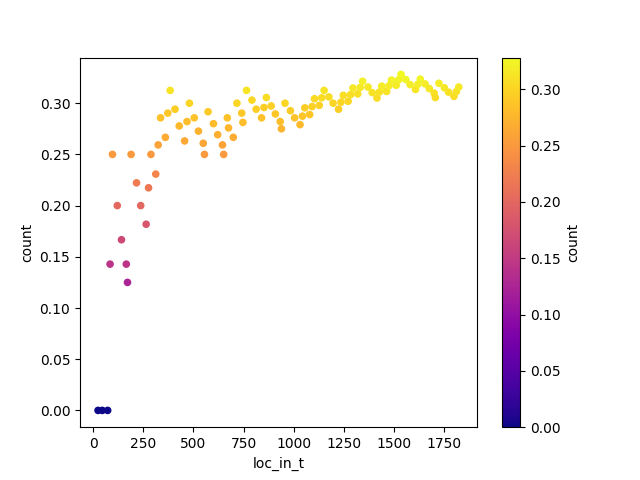
\includegraphics[scale=0.4]{lambda_ratio_from_data1_ones_100}
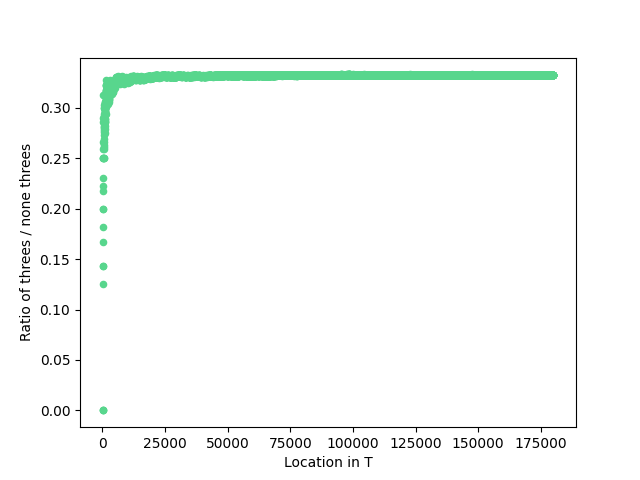
\includegraphics[scale=0.4]{lambda_ratio_from_data1_ones_10000}

\subsection{Primes Conjecture}
We observe that for any location X in T, where X is prime, the value of $\Lambda{(T_3)}$ is equal to 1.

\section{The Imbalance Of Zeroes And Ones}

The $T_3$ sequence begins $00000001000...,$ and the imbalance between zeroes and ones continues on. We sampled the ratio of zeroes to ones encountered in every third digit of the first $n$ digits of $T$ itself using a computer program, and found the following:

Ratio for the first $2^{10}$ digits: 2.8

Ratio for the first $2^{11}$ digits: 2.1045454545454545

Ratio for the first $2^{12}$ digits: 2.1045454545454545

Ratio for the first $2^{13}$ digits: 1.7282717282717284

Ratio for the first 2$^{14}$ digits: 1.7282717282717284

$\cdots$

Ratio for the first $2^{35}$ digits: 1.0228080103552828

The ratio does indeed appear to approach $1,$ but only very slowly -- even at over $10^{10}$ entries of $T_3$ computed, there are still ~2\% more zeroes than ones. The ratio does approach 1, but the imbalance between zeroes and ones grows forever.

\begin{definition}
\label{imb}
The imbalance function $d(n)$ is the number of zeroes minus the number of ones found in every third digit of the first $n$ digits of $T.$
\end{definition}

For example, $d(8)$ = 3, because the first eight digits of the Thue-Morse sequence are:
$$0, 1, 1, 0, 1, 0, 0, 1.$$
Taking every third digit, we have:
$$\textbf{0}, 1, 1, \textbf{0}, 1, 0, \textbf{0}, 1,$$
Which has three zeroes and no ones.

\subsection{Reversing Segment-Matching}

In Section 2, we developed the notion of the segment-matching method, which may be thought of more generally as a \emph{transformation} from a sequence in $T_3$ to one or more possible sequences in $T$ which would be its equivalent. However, we can also develop the opposite notion -- a transformation from $T$ to $T_3.$ Of course this is already possible:

$$[0]11[0]10[0]11[0]01[0] \cdots \rightarrow 00000 \cdots .$$

But we can invert the method to obtain a more useful transformation which uses \emph{every} digit in $T$ to create the corresponding sequence in $T_3.$ We may then apply this transformation to the \emph{whole} of the Thue-Morse sequence to better understand the $T_3$ sequence itself.

First, we can define three pairs of functions.

\begin{definition}
$\alpha_0(n)$ is the number of zeroes when counting every third element of the first $n$ digits of $T,$ starting on element 0. The number of ones encountered in the same manner is $\alpha_1(n).$
\end{definition}

\begin{definition}
$\beta_0(n)$ is the number of zeroes when counting every third element of the first $n$ digits of $T,$ starting on element 1, and the number of ones when counting in the same manner is $\beta_1(n).$
\end{definition}

\begin{definition}
$\gamma_0(n)$ is the number of zeroes when counting every third element of the first $n$ digits of $T,$ starting on element 2, and the number of ones when counting in the same manner is $\gamma_1(n).$
\end{definition}

Therefore, the imbalance function $d(n)$ is equal to $\alpha_0(n) - \alpha_1(n).$

We recall that the sequence

$$T_3(n), T_3(n+1), T_3(n+2), T_3(n+3), ...$$

for any positive integer $n$ which is a multiple of 4, is equivalent to

$$T(m), T(m), \overline{T(m+1)}, \overline{T(m+2)}, T(3), T(3), \overline{T(m+4)}, \overline{T(m+5)}, \cdots$$

for $m = 3n/4.$ Setting $n = m = 0,$ we see that the $T_3$ sequence itself is equal to:

$$T(0), T(0), \overline{T(1)}, \overline{T(2)}, \cdots$$

and so forth.

We now note that the above sequence truncated after the first $4n$ entries, which is the first $4n$ entries in $T_3$ for some positive integer $n,$ may be reordered as follows:

\begin{itemize}
\label{reorder}
\item Two copies of $T(3k)$ for each $k = 0 ... n - 1.$
\item One copy of $\overline{T(3k+1)}$ for each $k = 0 ... n - 1.$
\item One copy of $\overline{T(3k+2)}$ for each $k = 0 ... n - 1.$
\end{itemize}

We can see that the number of zeroes in the first $4n$ digits of $T_3,$ or $\alpha_0(12n),$ counts each zero in the first $3n$ digits of $T$ twice, assuming said zeroes have indices which are multiples of 3. The number of zeroes at every multiple of 3 in the first $3n$ digits of $T$ is equal to $\alpha_0(3n),$ and going down the rest of the bullet-point list we see that:

$$\alpha_0(12n) = 2 * \alpha_0(3n) + \beta_1(3n) + \gamma_1(3n).$$

Replacing $3n$ with $n,$ we see:

$$\alpha_0(4n) = 2 * \alpha_0(n) + \beta_1(n) + \gamma_1(n)$$

for all $n$ which is a multiple of $12$ (as this satisfies the requirement that $n$ is a multiple of 4 from above and that $n$ is a multiple of 3).
We also know that $n$ is even, so the total numbers of zeroes in the first $n$ digits of the Thue-Morse sequence is equal to the total number of ones, which are each equal to $n/2.$ We can then restate the above expression as:

$$\alpha_0(4n) = 2 * \alpha_0(n) + \frac{n}{2} - \alpha_1(n).$$

Likewise, we have:

$$\alpha_1(4n) = 2 * \alpha_1(n) + \frac{n}{2} - \alpha_0(n).$$

We can subtract these two expressions to get a value for $d(n)$ by Definition \ref{imb}:

\begin{lemma}
\label{ratiospec}
$d(4n) = 3 * d(n)$ for all numbers $n$ which are positive multiples of 12.
\end{lemma}

\begin{remark}
We can use this result to show roughly how fast the ratio of zeroes to ones decays. Let $r(n)$ denote $\alpha_0(n)/\alpha_1(n).$ The total size of $\alpha_0(k) + \alpha_1(k)$ is at most 1 away from $\frac{k}{3},$ we see that in the limit, $r(4k) - 1 \simeq \frac{3}{4} * (r(k) - 1).$
\end{remark}

\subsection{Imbalance Theorem}

We now have what we need to prove the Imbalance Theorem.

\begin{proof}

\begin{lemma}
\label{diff}
The difference $d(x+n) - d(n)$ has absolute value at most $n/3 + 1.$
\end{lemma}

\begin{proof}
Because the $\alpha(n)$ functions are defined as the number of zeroes and ones in every third term of the first $n$ terms of the Thue-Morse sequence, going from $x$ to $x+n$ adds at most $n/3 + 1$ terms to consideration, which adds at most $n/3 + 1$ terms to either the zero or the one tally.
\end{proof}

\begin{lemma}
\label{dip}
If $d(x)$ and $d(x+n)$ are both at least $m,$ and $x \leq y \leq x+n,$ then $d(y)$ is at least $m - n/6 - 1.$
\end{lemma}

\begin{proof}
Any point between $x$ and $x+n$ is at most $d/2$ apart from one of $x$ and $x+n,$ so by Lemma \ref{dip} its value must be at most $d/6 + 1$ less than $d$ evaluated at whichever of $x$ and $x+n$ it is closest to, which must by our assumption be at least $m.$
\end{proof}

\begin{lemma}
\label{x12}
Suppose $x$ is a positive multiple of $12.$ If $d(n) \geq 5$ for all $n$ such that $x \leq n \leq x+12,$ then $d(m) \geq 5$ for all $m$ such that $4x \leq m \leq 4x+48.$
\end{lemma}

\begin{proof}
Let $x$ be a multiple of $12$ such that $d(n)$ evaluated at any point from $x$ to $x+12$ is at least 5. By Lemma \ref{ratiospec} we know that $d(4x) \geq 15 \leq d(3x+48).$ Then by Lemma \ref{dip} we know that the minimum value of $d$ between $4x$ and $4x+48$ is at least $15 - (48/6) - 1,$ which is greater than $5.$
\end{proof}

\begin{lemma}
\label{4jump}
Let $x$ be a multiple of $12.$ If $d(n) \geq 5$ for all $n$ such that $x \leq n \leq 4x,$ then $d(m) \geq 5$ for all $m$ such that $4x \leq m \leq 16x.$
\end{lemma}

\begin{proof}
We see that $d(n) \geq 5$ for all multiples of 12 between $x$ and $4x,$ so by applying Lemma \ref{x12} to $x, x+12, \cdots 4x-12,$ we see that $d(n) \geq 5$ for all $m_1$ such that $4x \leq m_1 \leq 4x+48,$ for all $m_2$ such that $4x+48 \leq m_2 \leq 4x+96,$ and so forth.
\end{proof}

To wrap up the proof of the Imbalance Theorem, let $x$ be a multiple of $12$ such that $d(n) \geq 5$ for all $n$ such that $x \leq n \leq 4x.$ Then by Lemma \ref{4jump} and induction, we have that $d(n) \geq 5$ for all $n \geq x.$ Then, by showing $d(n) > 0$ for all $0 < n < x,$ we have proven the Imbalance Theorem.

A computer calculation shows that$d(n) \geq 5$ for all $n$ such that $24 \leq n \leq 96,$ and that $d(n) > 0$ for all $n$ such that $0 < n < 24.$ Therefore, the Imbalance Theorem is proven.
\end{proof}

\end{document}
